\section{Introduction} \label{sec:introduction}

Key aspects of the study of evolution, whether biological or digital, revolve around understanding the flow of genetic material among large populations of organisms.
As such, phylogenetic analyses assessing ancestry trees representing organsisms' evolutionary histories are a core tool in evolutionary biology.
In work with biological organisms, phylogenies are typically estimated through analysis of genetic similarities among organisms.
Although direct tracking is often preferable in \textit{in silico} experiments, in memory-constrained parallel and distributed computing contexts, applying reconstruction-based methods to track generate phylogeny trees can become advantageous.
As is also the case in biological studies, the efficacy of phylogenetic analysis in such \textit{in silico} work depends on efficient methods to generate accurate ancestry trees.
It is this topic we focus on in this work, presenting a novel trie-building algorithm that, in the scope of digital evolution, greatly improves the performance of phylogenetic reconstruction wile producing equivalent results compared to a naive approach.

\subsection{Applications of Phylogenetic Analysis}

Phylogenetic analyses provide key means to characterize and quantifying a broad array of evolutionary processes.
Clasically, these analyses have been applied to investigation of species-levewl macroevolutionary dynamics revolving around speciation and extinction rates; however, population- and organism-level dynamics can also be inferred, such as the spread of beneficial mutations within a population or fitness parameters like growth rate and probability of survival \citep{genthon2023cell, levy2015quantitative, stadler2013recovering}.
Phylogenetic analysis is also crucial in the field of epidemiology, playing a key role in informing public health interventions.
In this context, phylogenetic methods can be used to determine transmission history, pinpointing where and how chains of infection unfold \citep{wang2020role}.
In this vein, phylogenies are also key in assessing the prevalence of  ``super-spreader'' dynamics wherin disease spread is driven by a small set of high-risk individuals \citep{colijn2014phylogenetic}.

%\subsection{Phylogenies \& Digital Evolution} \label{sec:introduction:digital}

%In certain cases, however, the long runtime of biological evolution makes it infeasible to study; laboratory experiments may take years, or even decades, to complete -- a canonical example being the long-term evolution experiment \citep{wiser2013long}.
%Therefore, by simulating the behavior of a population, experiments can instead be done digitally, with simulations running in a fraction of the time.
%These systems can model key characteristics of biological populations, such as variation, natural selection, facilitation, movement, predation, and more.
%So, due to the nature of these simulations, conclusions about digital evolution can even be generalized to biological evolution \citep{pennock2007models, dolson2021digital}.

Phylogenies are also a valuable tool for analyzing evolutionary dynamics within digital evolution experiments.
In application-oriented contexts, phylogeny-based biodiversity metrics have been shown as predictive of solution quality outcomes for evolutionary computation-based optimization \citep{hernandez2022phylogenetic}.
Phylogeny-based methods can also be applied to characterize more general aspects of ecology, spatial structure, and selection pressure within \textit{in silico} populations \citep{moreno2023toward}.

Digital evolution approaches can also serve as a testbed to assess bioinformatics methodologies.
The Aevol\_4b system, for instance, uses a genetic system corresponding to that of DNA, allowing any genetic information to be processed using methods directly from bioinformatics \citep{daudey2024aevol}.
Likewise, population genetics work often incorporates SLiM, which supports sophisticated continuous-space modeling of single- and multi-species systems \citep{haller2023slim}.

\subsection{Reconstructing Phylogenies} \label{sec:introduction:reconst}

In biological studies, phylogenetic reconstruction methods typically work by assessing nucleotide changes between aligned DNA sequences from sample organisms.
Approaches include distance-based methods, where a distance matrix between organisms is computed and processed with methods such as neighbor-joining \citep{saitou1987neighbor}; or character-based methods, such as maximum-parsimony \citep{sober1991reconstructing}, which seeks to minimize the number of evolutionary changes necessary to explain an evolutionary history --- and maximum-likelihood \citep{felsenstein1981evolutionary}, which infers tree topologies maximizing a likelihood function \citep{de2014phylogenetic}.

Given the programmatic observability of digital simulations, digital evolution platforms typically incorporate direct tracking methods that record lineage ancestry as the simulation runs.
General-purpose phylogeny-tracking libraries exist for this purpose \citep{dolson2024phylotrack}, although many platforms simpli incorporate bespoke implementations into their own software \citep{ofria2004avida}.

In large-scale, many-processor simulations, however, challenges arise in managing a comprehensive record of ancestry.
To control memory use, it is typically necessary to trim away records of extinct lineages when performing direct tracking#
Detecting extinctions, however, introduces implementation complexity and overhead costs when lineage histories span across multiple processors.
Such an approach is also sensitive to data loss from crashed hardware or dropped messages, which has been highlighted as key consideration in achieving very large-scale artificial life systems \citep{ackley2016indefinite,ackley2014indefinitely}.
Challenges associated with comprehensive tracking are especially acute in specialized hardware accelerator devices, which represent a promising emerging direction in High-Performance Computing (HPC) \citep{emani2024democratizing}.
In incorporating thousands of processor cores per device, these hardware architecture impose trade-offs in memory capacity limitations and data locality restrictions that limit the feasibility of comprehensive tracking.
In such contexts, reconstruction-based approaches can provide an attractive balance between data fidelity anddata collection overhead.

\subsection{Hereditary Stratigraphy} \label{sec:introduction:hstrat}

\begin{figure*}

\centering
\begin{minipage}{0.75\textwidth}

\begin{minipage}{0.4\linewidth}
\centering
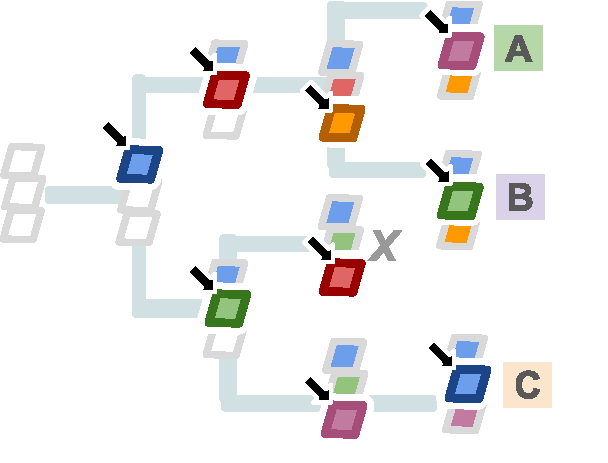
\includegraphics[height=1.5in]{img/hstratschematic-evolve}
\subcaption{evolve}
\end{minipage}%
\centering
\begin{minipage}{0.2\linewidth}
~~~

\includegraphics[height=1.5in]{img/hstratschematic-sample}
\subcaption{sample}
\end{minipage}%
\begin{minipage}{0.4\linewidth}
\centering
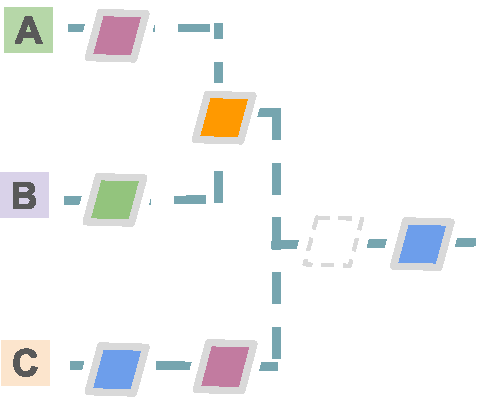
\includegraphics[height=1.5in]{img/hstratschematic-reconstruct}
\subcaption{reconstruct}
\end{minipage}
\end{minipage}%
\begin{minipage}{0.25\textwidth}
\caption{\textbf{TODO.}}
\label{fig:hstratschematic}
\end{minipage}

\end{figure*}

Under controlled conditions, such as laboratory experiments or evolution simulations, genetic material may be engineered to facilitate the accuracy and efficiency of estimating phylogenetic relatedness \citep{li2024reconstructing}.
In this vein, work with hereditary stratigraphy methods has sought to operate analogously, organizing genetic material to maximize reconstruction quality and minimize memory footprint \citep{moreno2022hereditary}.
Hstrat material can be bundled with agent genomes in a manner akin to non-coding DNA, entirely neutral with respect to agent traits and fitness.

HStrat associates each generation along each lineage with an identifying ``fingerprint'' marker, referred to as a differentia.
On birth, offspring receive a new differentia value and append it to an inherited chronological record of past values, each corresponding to a generation along that lineage.
Under this scheme, mismatching differentia can be used to delimit the extent of common ancestry.
Figure \ref{fig:hstratschematic} gives a schematic overview of the hereditary stratigraphy approach.

To save space, differentiae may be pruned away -- although, at the cost of reducing precision in inferring relatedness.
Reducing the number of bits per differentia can also provide many-fold memory space savings.
Using single bits or single bytes is appropriate for most use cases.

% and the possibility of collisions and missing data.
Inferring relatedness from biological sequence data can be a highly challenging and computationally-intensive problem \citep{miller2010creating}.
The structured marker data used in hereditary stratigraphy somewhat ameliorates this challenge by allowing phylogeny reconstruction to be approached as a trie-building procedure of identifying common string prefixes \citep{delabriandais1959file,moreno2024analysis}.
However, the presence of missing data due to differentia dropped to save memory complicates matters.
In the context of trie-building, markers possessed by only a subset of organisms effectively act as ``wildcard'' characters for organisms that do not possess them, possibly having taken on any differentia value.
Therefore, placing an organism on a trie requires evaluating possible subsequent paths following the wildcard to identify further matches.
With the possibility of differentia value collisions with small differentia sizes (e.g., 1 bit), identifying the best-matching path after a wildcard missing value can require looking ahead several consecutive markers.
Furthermore, where consecutive wildcards are encountered, the number of possible paths that must be explored can grow exponentially.
% resolving these wildcards can require possibly-exponential evaluation of alternate trie paths.
% briefly mentions the naive trie-based approach we improve upon here, and remarks upon the wildcard matching problem associated with it \citep{moreno2024analysis}.

%TODO cite ackley2023robust for barcodes

% Phylogeny inference is
% A naive approach requires...

Although previous work has investigated the quality of phylogenies constructed from hereditary stratigraphy data using trie-based approaches \citep{moreno2025testing}, the computational intensity of the naive wildcard-matching approach has limited the scale of phylogenetic reconstructions practical to work with and restricted experimental throughput for smaller reconstructions.
Given the objective of the methodology to facilitate studying very large scale digital evolution experiments, achieving reconstruction efficiency sufficient to collect large-scale phylogeny data is critical to the overall utility of the methodology in enabling observable experiments.
In this work, we develop algorithms for more efficient trie reconstruction in the face of missing data and explore their practical scalability through benchmark trials of high-performance implementations.

The following section introduces our proposed ``shortcut'' algorithm for the trie building approach explored in this paper. We then describe a set of methods to validate reconstruction quality and test empirical scaling behavior and performance on to billion-genome-scale workloads.

% \citet{moreno2024trackable} used the naive trie building algorithms, and is the base for the benchmarking code that we did here (but we add some etensions here).
% The trees built in this work were only TODO tips.
% 

% Earliest work with hereditary stratigraphy used a very simple UPGMA/neighbor joining approaches based on estimations of pairwise distance beteen taxa \citet{moreno2022hereditary}.

% The end result is the genetic information of an organism being a series of rank-differentia pairs, where each rank represents a generation at which a datum was retained, and the differentia representing the datum itself.
% However, the presence of missing information is a hurdle that a phylogenetic reconstruction algorithm must overcome, and may cause significant slowdowns using traditional algorithms.

% Given the various work that has been done on hereditary stratigraphy, it is useful to overview the recent work and to highlight how present work differs from it.

% \citet{moreno2022hereditary} introduced the general hereditary stratigraphy method, which was implemented in a accompanying software package \citep{moreno2022hstrat}.
% \citet{moreno2023toward} investigated the nature of phylostatistical fingerprints left by evolutionary forces of ecology, selection pressure, and spatial structure, and the effects of approximation error from hereditary stratigraphy on detecting these fingerprints.
% \citet{moreno2024methods} explored how the methodology might be extended from asexual systems, which we focus on here, to sexual systems through gene tree tracking and gene drive mechanisms.

% \citet{moreno2024structured} introduced the ``surface'' data structure which is used in this work, taking a generalized ring buffer approach to storing differentia data \citet{gunther2014algorithm}.
% The original trie-based reconstruction method is used in

% \textbf{TODO add more about hstrat} 

% \subsection{Problem Statement} \label{sec:introduction:problem}

% TODO @mmore500

% Unfortunately, the existing naive algorithm is simply not fast enough for large-scale simulations, with 


% @MAM I moved the following content into the "algorithm" section in the "naive trie building algorithm" subsection.
% I think what we want here is something that is going to be a tricky mix of vague and specific
% ... maybe a good term is "evocative"
% we want to evoke the core problem by describing "what" the challenge is rather than exactly "how" or "why"
% and we can end with "A more detailed description of the challenge solved in this work is provided in Section \ref{sec:algorithm}...

